\subsection{Dedekind Cuts: Defining the Real Line Into Existence}

Dedekind’s genius was not in discovering irrational numbers, but in \textbf{defining them into existence}.

Before Dedekind, irrationals were treated like mysterious invaders—quantities that snuck into mathematics through geometry or approximation, but never quite fit into the clean logic of arithmetic. You could draw \( \sqrt{2} \) on a diagonal, or compute its decimal expansion to a hundred digits—but what \emph{was} it, really?

Dedekind answered with breathtaking clarity: irrational numbers aren’t intruders in the number system. They are \textbf{the boundaries that rational numbers leave behind}.

\medskip

A \textbf{Dedekind cut} is a way of partitioning the rational numbers \( \mathbb{Q} \) into two sets \( A \) and \( B \) such that:

\begin{itemize}
  \item Every element of \( A \) is less than every element of \( B \)
  \item \( A \) contains no greatest element
\end{itemize}

That \emph{cut} — the knife-edge between the two sets — is what we define as a real number. If the cut lands on a rational number, like \( 5 \), then the number it defines is \( 5 \). But if the cut \emph{misses} every rational number—say, if \( A \) is the set of all rationals whose square is less than 2—then it still defines a precise location. That location, though unoccupied by any rational, is what we call \( \sqrt{2} \).

\medskip

The brilliance here is that Dedekind didn’t need to construct irrational numbers from scratch. He didn’t build \( \sqrt{2} \) out of sequences or decimal expansions. Instead, he showed that irrational numbers were \emph{already encoded} in the rational line—as \textbf{missing endpoints}, as \textbf{logical limits}, as \textbf{absences that demand acknowledgment}.

In doing so, Dedekind transformed the real number line from a computational tool into a philosophical structure. The continuum wasn’t just a blur of digits—it became a complete, gapless terrain. Every point, whether rational or not, could be named, located, and logically justified.

\begin{quote}
Irrational numbers are not exceptions—they are \emph{expectations} that the rationals fail to meet.
\end{quote}

Dedekind’s cuts filled in those gaps not with approximations, but with certainty.


\begin{figure}[H]
    \centering
    % File: dedekind_cut_figure.tex
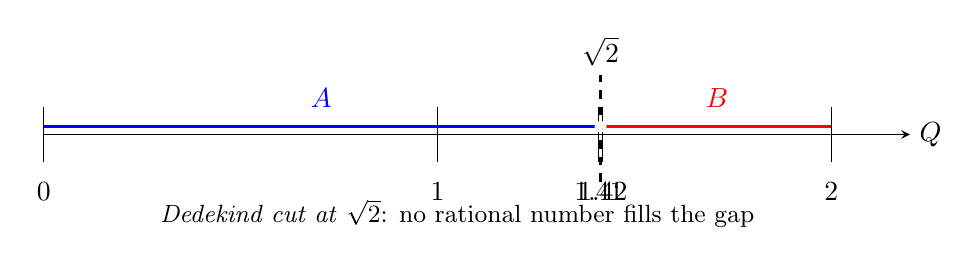
\begin{tikzpicture}[scale=5, >=stealth]
    \draw[->] (0,0) -- (2.2,0) node[right] {\(\mathbb{Q}\)};
    \foreach \x/\label in {0/0, 1/1, 1.41/1.41, 1.42/1.42, 2/2} {
      \draw[shift={(\x,0)}] (0pt,2pt) -- (0pt,-2pt) node[below=4pt] {\(\label\)};
    }
    \draw[very thick, blue] (0,0.02) -- (1.41,0.02) node[midway, above=3pt, blue] {\(A\)};
    \draw[very thick, red] (1.42,0.02) -- (2,0.02) node[midway, above=3pt, red] {\(B\)};
    \draw[dashed, thick] (1.4142, -0.12) -- (1.4142, 0.15);
    \node[above] at (1.4142, 0.15) {\(\sqrt{2}\)};
    \filldraw[white] (1.4142,0.02) circle (0.4pt);
    \node at (1.05, -0.2) {\small \textit{Dedekind cut at} \(\sqrt{2}\): no rational number fills the gap};
\end{tikzpicture}
    \caption{A Dedekind cut at \( \sqrt{2} \): the rational numbers are split into two sets \( A \) and \( B \), with no greatest element in \( A \), and no smallest in \( B \). The cut defines a real number.}
  \end{figure}





\begin{figure}[H]
    \centering
    \begin{tikzpicture}[xscale=125, yscale=7.5, >=stealth] % 25% larger than xscale=100, yscale=6
    
      % Baseline height
      \def\baseline{1.6}
    
      % Extended number line
      \draw[->] (1.36, \baseline) -- (1.45, \baseline) node[right] {\(\mathbb{Q}\)};
    
      % Main tick marks and labels (1.45 shifted right slightly)
      \foreach \x/\label in {
        1.36/1.36, 1.37/1.37, 1.38/1.38, 1.39/1.39,
        1.40/1.40, 1.41/1.41, 1.42/1.42, 1.43/1.43, 1.44/1.44
      } {
        \draw[thick] (\x, \baseline-0.02) -- (\x, \baseline+0.02);
        \node[below=4pt, font=\scriptsize] at (\x, \baseline) {\(\label\)};
      }
    
      % Shifted label for 1.45
      \draw[thick] (1.45, \baseline-0.02) -- (1.45, \baseline+0.02);
      \node[below right=2pt and -2pt, font=\scriptsize] at (1.45, \baseline) {\(1.45\)};
    
      % Tiny-scale ticks near sqrt(2)
      \foreach \x in {1.414, 1.4142, 1.415} {
        \draw[thick] (\x, \baseline-0.02) -- (\x, \baseline+0.02);
      }
    
      % Arrows to closely spaced numbers near sqrt(2)
      \draw[->, thin] (1.375, \baseline - 0.23) -- (1.414, \baseline - 0.01);
      \node[below=1.7cm, font=\scriptsize] at (1.375, \baseline) {\(1.414\)};
    
      %\draw[->, thin] (1.385, \baseline - 0.25) -- (1.4142, \baseline - 0.01);
      %\node[below=1.7cm, font=\scriptsize] at (1.385, \baseline) {\(1.4142\)};
    
      \draw[->, thin] (1.455, \baseline - 0.23) -- (1.415, \baseline - 0.01);
      \node[below=1.7cm, font=\scriptsize] at (1.455, \baseline) {\(1.415\)};
    
      % Dedekind cut: sets A and B
      \draw[very thick, blue] (1.36,\baseline+0.06) -- (1.41421,\baseline+0.06) node[midway, above=2pt, blue] {\(A\)};
      \draw[very thick, red] (1.41423,\baseline+0.06) -- (1.45,\baseline+0.06) node[midway, above=2pt, red] {\(B\)};
    
      % Dashed line at sqrt(2)
      \draw[dashed, thick] (1.41421356, \baseline-0.1) -- (1.41421356, \baseline+0.25);
      \node[above] at (1.41421356, \baseline+0.25) {\(\sqrt{2}\)};
      \filldraw[white] (1.41421356,\baseline+0.06) circle (0.5pt); % visual cut
    
      % Caption
      \node at (1.405, \baseline - 0.4) {\small \textit{Zoomed Dedekind cut around \( \sqrt{2} \) with nearby rational approximations.}};
    
    \end{tikzpicture}
    \caption{Dedekind cut showing how \( \sqrt{2} \) slices the rational number line.}
\end{figure}
    
    
    
    
    
    
    
    
    
    



\begin{tcolorbox}[colback=gray!5!white, colframe=black!75!white, title={Sidebar: Dedekind Cuts vs. Decimal Expansions}]
    \textbf{Decimal Expansions:}\\
    Decimal representations like \( 3.14159\ldots \) offer a convenient way to \emph{approximate} real numbers. They are:
    \begin{itemize}
      \item Familiar and intuitive
      \item Easy to compute with
      \item Base-dependent (e.g., base-10, base-2)
    \end{itemize}
    However, they suffer from ambiguity: e.g., \( 0.999\ldots = 1.0 \). Moreover, they require infinite sequences to represent irrationals—useful for calculation, but not for rigorous definition.
    
    \medskip
    
    \textbf{Dedekind Cuts:}\\
    Introduced by \textbf{Richard Dedekind} in 1872, a Dedekind cut defines a real number as a partition of the rational numbers into two sets \( A \) and \( B \) such that:
    \begin{itemize}
      \item Every element of \( A \) is less than every element of \( B \)
      \item \( A \) has no greatest element
    \end{itemize}
    This construction is:
    \begin{itemize}
      \item Base-independent
      \item Rigorous and logically complete
      \item Capable of defining irrationals directly
    \end{itemize}
    
    \textbf{Dedekind’s View:} Decimal expansions are helpful representations, but they don't define what real numbers \emph{are}. Cuts, he argued, express the \textbf{continuity} of the number line with mathematical precision.
    
\end{tcolorbox}
